\usetikzlibrary{calc}
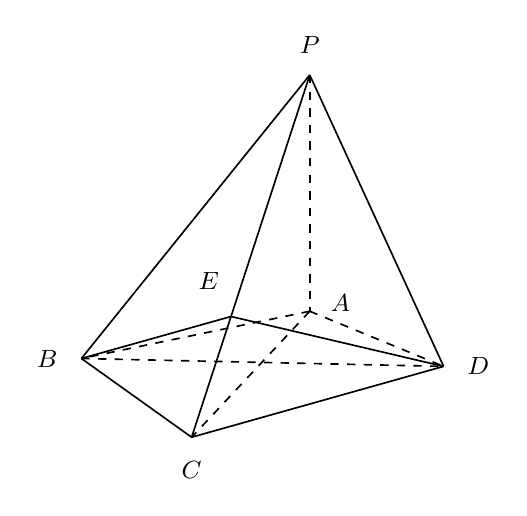
\begin{tikzpicture}[line width=.6pt, font=\small, x=1cm, y=1cm]
\coordinate (P) at (2.9000000000,4.6000000000);
\coordinate (A) at (2.9,1.6);
\coordinate (B) at (0,1.0);
\coordinate (C) at (1.4,0);
\coordinate (D) at (4.6,0.9);
\coordinate (E) at (1.9000000000,1.5333333333);
\draw (P)--(B);
\draw (P)--(D);
\draw (P)--(C);
\draw[dashed] (P)--(A);
\draw (B)--(C)--(D);
\draw (B)--(E);
\draw (E)--(D);
\draw[dashed] (B)--(D);
\draw[dashed] (A)--(B);
\draw[dashed] (A)--(C);
\draw[dashed] (A)--(D);

\node[above=4pt] at (P) {$P$};
\node[right=5pt,xshift=-1pt,yshift=3pt] at (A) {$A$};
\node[left=5pt] at (B) {$B$};
\node[below=5pt] at (C) {$C$};
\node[right=5pt] at (D) {$D$};
\node[left=6pt,above=2pt,xshift=-2pt,yshift=4pt] at (E) {$E$};
\end{tikzpicture}
